%% The following is a directive for TeXShop to indicate the main file
%%!TEX root = diss.tex

\chapter{Results}
\label{ch:Results}
At this stage in my thesis project, I have created the fast simulation and included all of the necessary optical effects. The features that I have and have not yet implemented are discussed further in the Methods section. As I talk about later in this section, I have started determining the effectiveness of the simulation and comparing it to the preexisting Geant4 simulation, although work for these tasks is ongoing.

\section{Comparison with Geant4} 
In this section, I will compare the simulated photon distribution between my simulation and the full Geant4 simulation.
They will be compared on a number of metrics, including the number of photons detected in the photon ring, and the level of background photons (determined by taking the ratio of histograms simulated by my simulation and by Geant4). This work is in progress: comparisons have been done, but it is still necessary to more accurately quantify the differences between the two simulations and display these results. I will describe the differences between my simulation and the full Geant4 simulation, and make the claim that my simulation contains enough of the necessary physics to simulate Cherenkov photons with sufficient accuracy for our purposes.

\section{Particle Separation}
In this section, I will talk about how well the likelihood approach using my simulation differentiates between different particles. 
Charged pions have a mass of  0.140 GeV, charged kaons have a mass of 0.494 GeV, and protons have a mass of 0.938 GeV.
Because of this, it is particularly hard to distinguish between pions and kaons, but easier to distinguish protons from kaons, and easier still to distinguish protons from pions.

Let's suppose we want to see how well this likelihood approach works on a particle that is 7 GeV and measured to be at the origin and travelling directly in the z-direction.
To check the certainty with which we can determine whether this is a pion or kaon, we would follow this approach:

\begin{enumerate}
\item Generate 10,000 pions with these values in Geant4, project the generated photons onto a detector, apply efficiency corrections, and store the resulting histogram of detected photon hits for each pion. 
\item Do the same, but with kaons instead of pions
\item Given the particle initial position, initial direction, and momentum, we use my simulation to generate two photon probability distribution histograms, corresponding to pions or kaons
\item For each event simulated in Geant4, we compute the log likelihood of the histogram with respect to each of the 3 photon probability distribution functions.
\item For each true particle type, we plot a histogram of the log of the ratio of likelihoods between the two hypotheses.
This is just the differences between the log-likelihoods of the two hypotheses.
\item We look at the separation between the distributions: this is equal to the difference in means between the distributions, divided by the RMS of each distribution added in quadrature
\end{enumerate}

The result of this procedure is shown in Figure \ref{fig:kaonpionsep}. The two distributions are separated by a distance of $2.4 \sigma$ - the significant overlap between the two distribution indicates that there is a relatively high chance of misidentification. Applying the same procedure to verify our separation between kaons and protons gives the results shown in Figure \ref{fig:kaonprotonsep}. Here we see that the two distributions do not significantly overlap and have a separation of $4.7 \sigma$, meaning that at this momentum and angle, protons are very unlikely to be misidentified as kaons, and vice versa.
\begin{figure}[]
\centering
\resizebox{0.9\textwidth}{!}{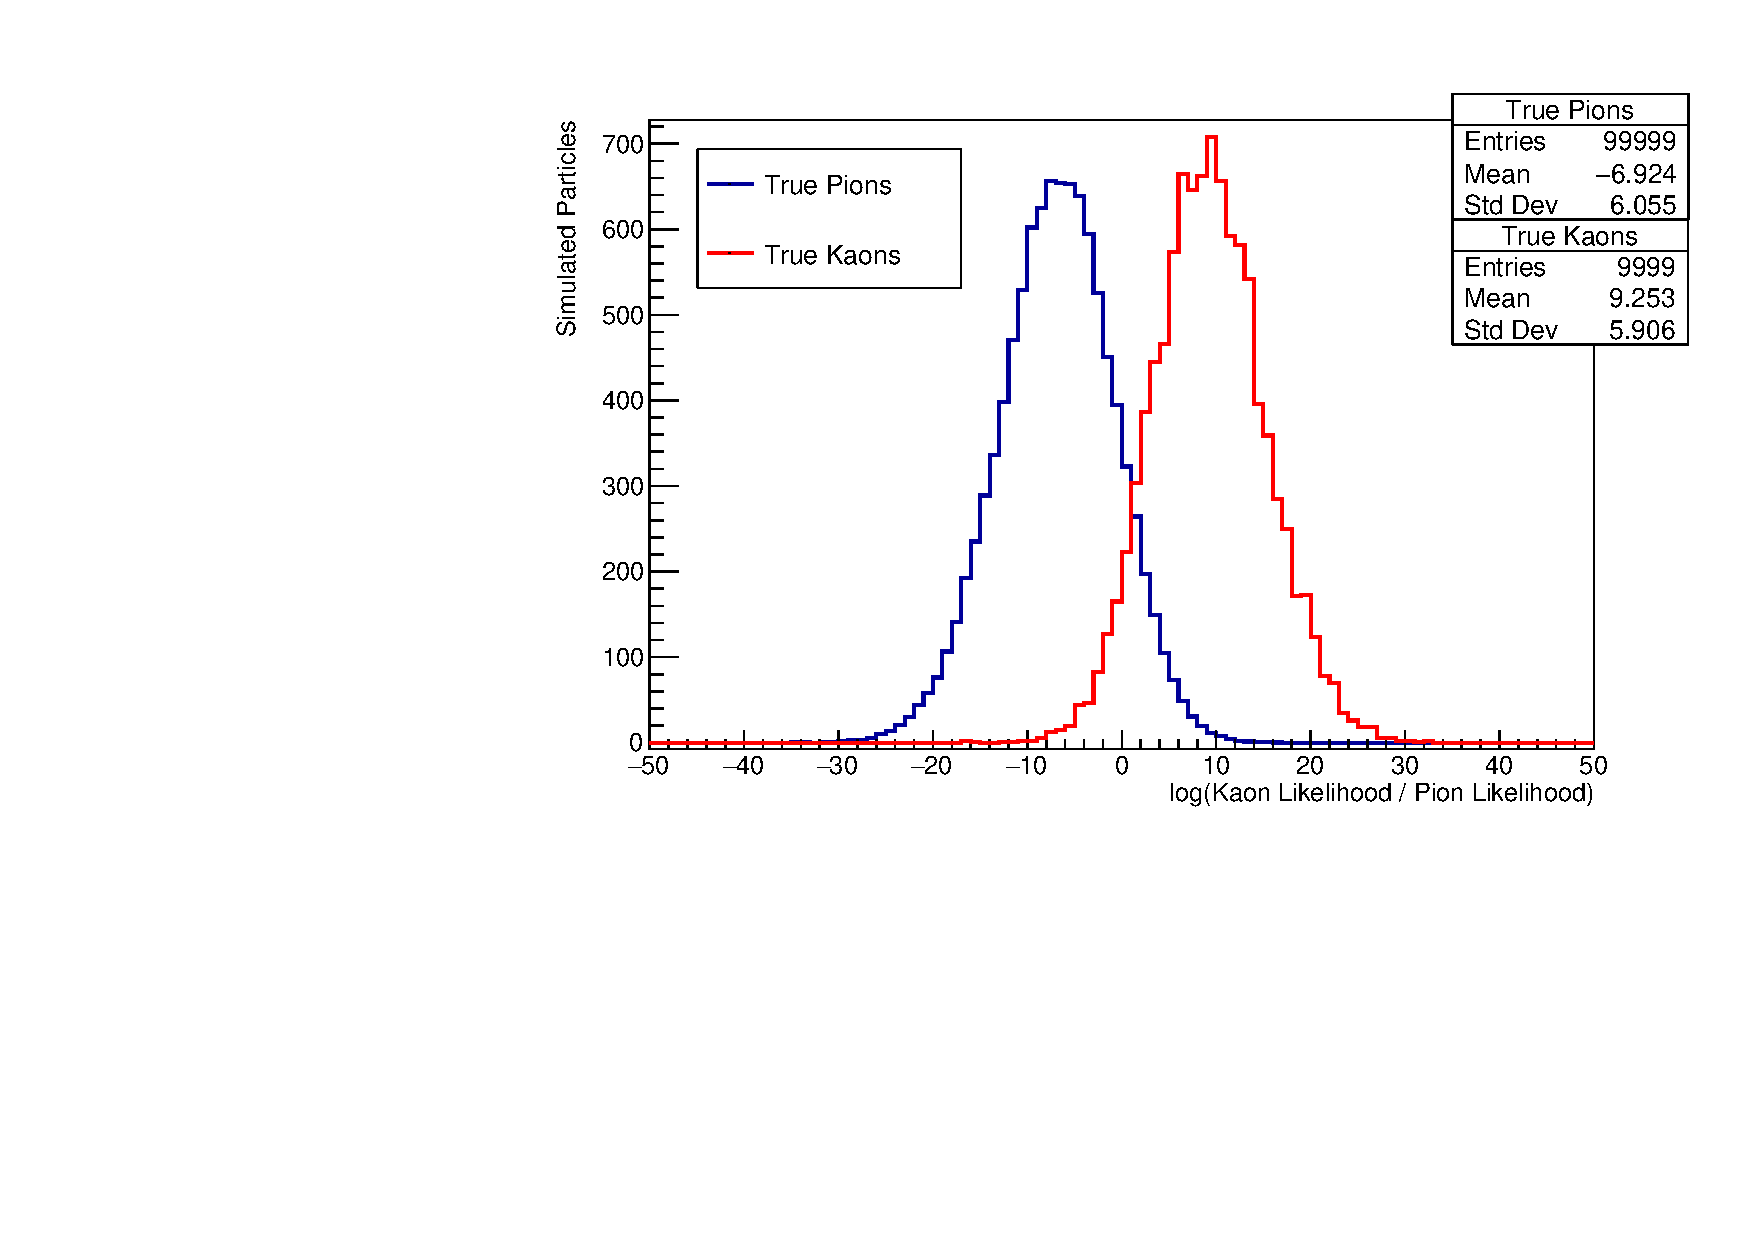
\includegraphics{./figs/kaonPionSep.pdf}}
\caption[Particle identification separation for 7 GeV pions and kaons]{Histogram showing the logarithm of the ratios of likelihoods between kaons and pions for both ``true" kaons and ``true" pions. The two distributions have a separation of 2.4 $\sigma$.}
\label{fig:kaonpionsep} 
\end{figure}

\begin{figure}[]
\centering
\resizebox{0.9\textwidth}{!}{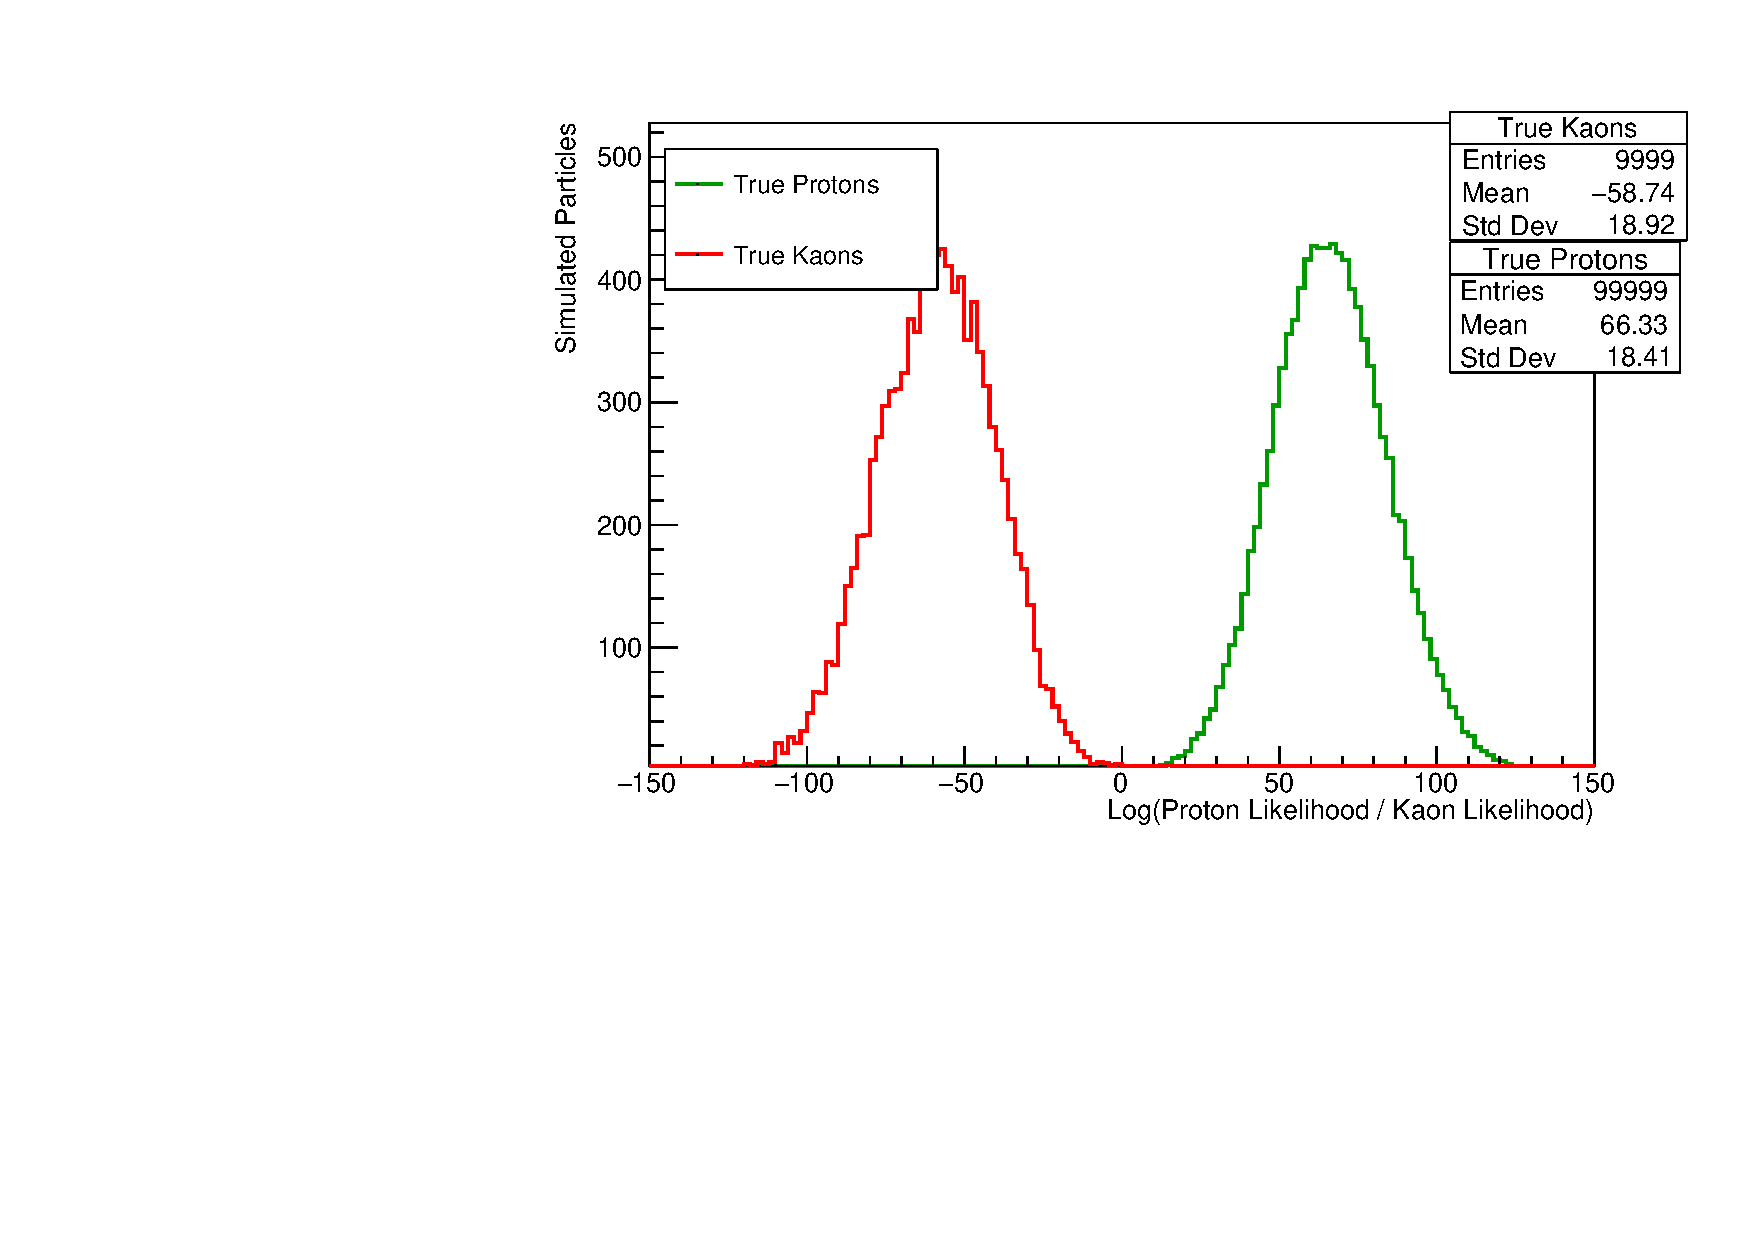
\includegraphics{./figs/kaonProtonSep.pdf}}
\caption[Particle identification separation for 7 GeV kaons and protons]{Histogram showing the logarithm of the ratios of likelihoods between protons and kaons for both ``true" protons and ``true" kaons. The two distributions have a separation of  4.7 $\sigma$.}
\label{fig:kaonprotonsep} 
\end{figure}

\TODO{While I have examined these results for 7 GeV pions, kaons, and protons, I still must check the separation for: \\
- Different initial particle directions and positions \\
- Different momenta \\
- Multi-particle events
}

\endinput

Any text after an \endinput is ignored.
You could put scraps here or things in progress.
